\documentclass[../_main/handlingar.tex]{subfiles}

\begin{document}
\motion{Äskning av pengar för inköp av ny tandemcykel}

Tandemstafetten är och har alltid varit ett evenemang som lockat många av E-sektionens
medlemmar. Under 2019 års upplaga så hade sektionen flest deltagare av alla sektioner på
LTH och vann även priset ”flest obrukbara cyklar”. Vi hade inte bara sönder vår egen cykel
utan även V-sektionens cykel. E-sektionen har i dagsläget två cyklar som båda är trasiga trots
den stora mängd kärlek de har fått.

\begin{center}
    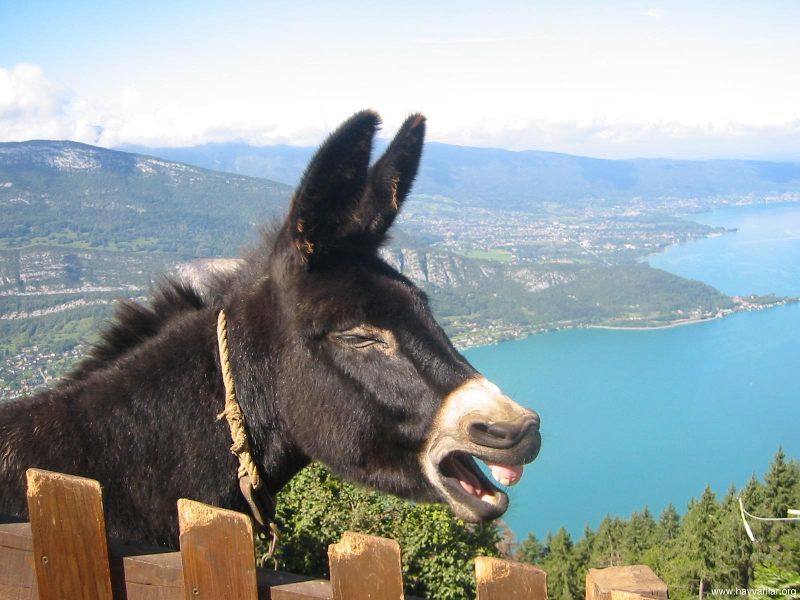
\includegraphics[width=10cm]{esek.jpg}
\end{center}

Därför yrkar vi på
\begin{attsatser}
    \att köpa in en ny tandemcykel till sektionen,
    \att budget sätts till 11 000 kr,
    %\att under \S0 i stadgarna lägga till\par
    %\begin{itshape}
    %    ``att'':
    %    \begin{itemizedash}
    %        \item att
    %        \item \sout{att}
    %        \item \hl{att}
    %    \end{itemizedash}
    %\end{itshape}
    \att kostnaden belastar utrustningsfonden, samt
    \att detta läggs på beslutsuppföljningen till (vårtermins) med undertecknad som ansvarig.
\end{attsatser}

Länk till potentiellt köp: https://www.sportfritid.se/monark-tandem-3-vxl.html

\begin{signatures}{2}
    \mvh
    \signature{Simon Mahdavi}{Vice Entertainer}
    \signature{Casper Schwerin}{Vice Entertainer}
\end{signatures}

\end{document}
